\documentclass{article}
\usepackage[english]{babel}
\usepackage{amsmath,amssymb,graphicx,enumerate,hyperref,calc,ifthen,tabularx,capt-of}

%%%%%%%%%% Start TeXmacs macros
\newcommand{\tmaffiliation}[1]{\\ #1}
\newcommand{\tmop}[1]{\ensuremath{\operatorname{#1}}}
\newcommand{\tmstrong}[1]{\textbf{#1}}
\newcommand{\tmtextup}[1]{\text{{\upshape{#1}}}}
\newenvironment{enumeratenumeric}{\begin{enumerate}[1.] }{\end{enumerate}}
\newenvironment{enumerateroman}{\begin{enumerate}[i.] }{\end{enumerate}}
\newenvironment{itemizedot}{\begin{itemize} \renewcommand{\labelitemi}{$\bullet$}\renewcommand{\labelitemii}{$\bullet$}\renewcommand{\labelitemiii}{$\bullet$}\renewcommand{\labelitemiv}{$\bullet$}}{\end{itemize}}
\newenvironment{tmindent}{\begin{tmparmod}{1.5em}{0pt}{0pt}}{\end{tmparmod}}
\newenvironment{tmparmod}[3]{\begin{list}{}{\setlength{\topsep}{0pt}\setlength{\leftmargin}{#1}\setlength{\rightmargin}{#2}\setlength{\parindent}{#3}\setlength{\listparindent}{\parindent}\setlength{\itemindent}{\parindent}\setlength{\parsep}{\parskip}} \item[]}{\end{list}}
\newenvironment{tmparsep}[1]{\begingroup\setlength{\parskip}{#1}}{\endgroup}
\newcounter{tmcounter}
\newcommand{\custombinding}[1]{%
  \setcounter{tmcounter}{#1}%
  \addtocounter{tmcounter}{-1}%
  \refstepcounter{tmcounter}}
\newcommand{\tmfloatcontents}{}
\newlength{\tmfloatwidth}
\newcommand{\tmfloat}[5]{
  \renewcommand{\tmfloatcontents}{#4}
  \setlength{\tmfloatwidth}{\widthof{\tmfloatcontents}+1in}
  \ifthenelse{\equal{#2}{small}}
    {\setlength{\tmfloatwidth}{0.45\linewidth}}
    {\setlength{\tmfloatwidth}{\linewidth}}
  \begin{minipage}[#1]{\tmfloatwidth}
    \begin{center}
      \tmfloatcontents
      \captionof{#3}{#5}
    \end{center}
  \end{minipage}}
%%%%%%%%%% End TeXmacs macros

\begin{document}

\raisebox{0.0\height}{
\includegraphics[width=14.8741637150728cm,height=2.73051948051948cm]{protocol-1.pdf}}

ECMI Modelling Week 2023

University of Szeged, Bolyai Institute

\

\

\

\title{Application of data-driven models in hydrological forecasting}

\author{
  
  \tmaffiliation{Zsolt Vizi (University of Szeged, Hungary)\\
  P{\'e}ter Koz{\'a}k (Water Management Directorate of Als{\'o}-Tisza,
  Hungary)\\
  \\
  Auer Lorenz (JKU, Austria)\\
  Endr{\'e}sz Bal{\'a}zs (BME, Hungary)\\
  Mitlas{\'o}czki Endre (University of Szeged, Hungary)\\
  Scharnreitner Franz (JKU, Austria)\\
  Tammi Aleksis (University of Eastern Finnland, Finnland)}
}

\maketitle

\

\

\

\

\

\

\

\

\

\

\

\

\

\


\[ \tmop{August} 29, 2023 \]
{\newpage}

{\tableofcontents}

{\newpage}

\section{Introduction}

Szeged is often called City of Sunshine, and yet the people from Szeged often
have to worry about too high water levels. The Tisza river flowing through the
city, has historically brought several devastating floods to the citizens of
Szeged. The goal of our project was to create an algorithm that can predict
the water levels for the next week. Of course there have been several, very
promising attempts at this before, each with its own benefits and flaws. Some
of the tricky aspects of this problem include the ever changing river bed, the
very shallow slope of the Tisza and incomplete data due to measurement
stations being constructed/removed. In a recent paper{\cite{WaterLevel2023}},
co-authored by our instructor, they used an ML model to accurately and very
cost efficiently predict the water levels in Szeged for the next 7 days.
During the ECMI Modelling Week 2023 our team of five students, with the lead
of our instructor Zsolt Vizi, further explored this approach, leading to
promising and interesting results.

\section{Report}

The data, our instructors provided us, consisted of water level measurements
at several points of the river Tisza before as well as after Szeged. Figure
\ref{map} shows a map of all the 56 measurement stations (blue, green, red) in
the original dataset, as well as several upstream dams (yellow). Most of the
stations are along the main stem of the river Tisza, which originates in the
north of Szeged. However there are also several stations along tributaries.
Notably the dataset also features 3 stations past Szeged. These are of
importance as the slope of the Tisza is very shallow. If the Danube, which the
Tisza flows into, carries more water than usual, the water of the Tisza can
not discharge at its usual rate. This is the reason why the floods of the
Tisza river often last several weeks. The dataset contains daily measurements
starting in 1951 up until 2020. The two biggest floods contained in the
dataset were in the years 1970 and 2006, each of them lasting roughly one
month.

\

\begin{figure}[h]
  \raisebox{0.0\height}{
\includegraphics[width=7.4370818575364cm,height=11.4316214088941cm]{protocol-2.pdf}}
  \caption{Map of measurement stations (green and red), dams (yellow) and
  Szeged (blue)\label{map}}
\end{figure}

\subsection{Overview}

We devided our work into several stages. Each of which will be described by
one of the following chapters in more detail.
\begin{enumeratenumeric}
  \item cleaning the data
  
  \item splitting the data
  
  \item data imputation
  
  \item reducing dimensionality
  
  \item choosing a model
  
  \item implementation
  
  \item verification of results
\end{enumeratenumeric}
\subsection{Cleaning the data}\label{clean}

The dataset, which contains the daily water levels of each station, has some
holes. Maybe a station was not yet built, the station was destroyed in a flood
or the worker noting the values was inconsistent. Also the river changes over
time and old data might not be as reliable as one might hope for.

\begin{figure}[h]
  \raisebox{0.0\height}{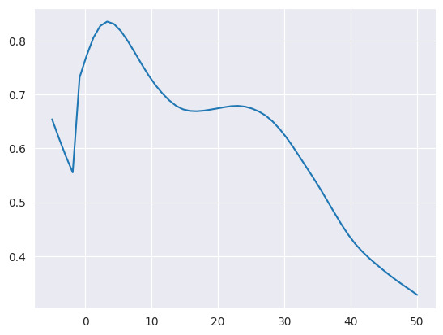
\includegraphics[width=14.8741637150728cm,height=1.55942542306179cm]{protocol-3.pdf}}
  \caption{Visual representation of the holes in the data from 1951 (left) to
  2020 (right)}
\end{figure}

Due to this we want to choose the stations as well as the time frame of data
to use, for training and validation, carefully. We also need to find a way to
fill the remaining holes in the data. (see chapter \ref{imputation})

As we want our model to be practical, we have to exclude all measurement
stations, which are not in use today. Also if a station started recording no
more than several weeks ago, its data will not be useful right now, as we
would have to fill in most of its holes. Data, we fill the holes with, will at
best not influence the result. There is no way for filled in data to provide
new, useful and correct insights.

Following this logic, we exclude stations with very big amounts of missing
data. The threshold we choose is more than 50\% missing datapoints. This
leaves us with a reduced dataset of 48 stations.

\begin{figure}[h]
  \raisebox{0.0\height}{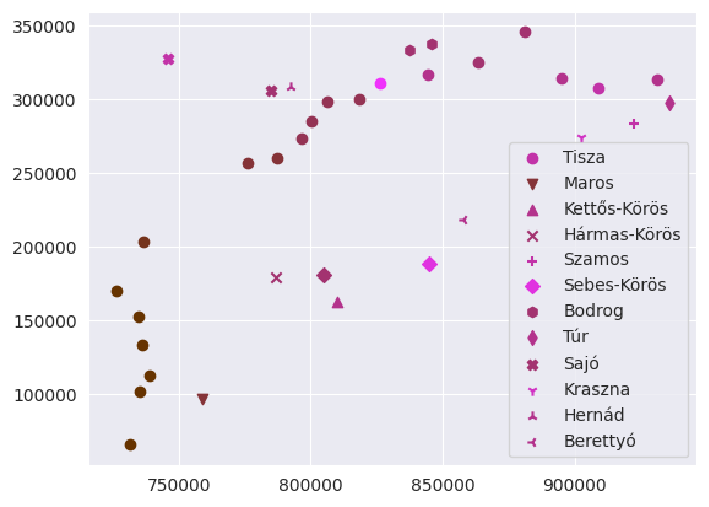
\includegraphics[width=14.8741637150728cm,height=1.5734126984127cm]{protocol-4.pdf}}
  \caption{Visual representation of the holes in the reduced dataset}
\end{figure}

Note that there are still holes in the dataset. If we would cut every station
with incomplete data, that would only leave us with around a dozen stations.

\subsection{Splitting the data}

As the riverbed constantly changes (e.g. erosion, floods, dams), we want to
choose the training data with that in mind. For instance, if we would do the
usual 80/20 spilt of training and validation data, so, train on the older 80\%
and validate on the newer 20\%, then the model mostly knows how to predict
floods from 50 years ago. Would it perform much worse with newer floods, if
the river system had changed?

To get an idea on how to spilt the data, we did research on the dams (table
\ref{dams}) and dams (table \ref{floods}) of the Tisza.

\begin{table}[h]
  \begin{tabular}{|l|l|l|l|l|}
    \hline
    Name & since & lon. & lat. & Wattage\\
    \hline
    Gib{\'a}rti v{\'i}zer{\H o}m{\H u} & 1903 & 48.317944 & 21.1635 & 1000\\
    \hline
    Fels{\H o}dobszai v{\'i}zer{\H o}m{\H u} & 1911 & 48.263687 & 21.084688 &
    940\\
    \hline
    B{\'e}k{\'e}sszentandr{\'a}si duzzaszt{\'o} & 1942 & 46.891 & 20.4995 &
    2000\\
    \hline
    Keszny{\'e}teni v{\'i}zer{\H o}m{\H u} & 1945 & 47.99597 & 21.033205 &
    4400\\
    \hline
    Tiszal{\"o}ki v{\'i}zer{\H o}m{\H u} & 1959 & 48.025141 & 21.307876 &
    12900\\
    \hline
    Kisk{\"o}rei v{\'i}zer{\H o}m{\H u} & 1973 & 47.492961 & 20.515569 &
    28000\\
    \hline
  \end{tabular}
  \caption{\label{dams}General information about the dams }
\end{table}

\begin{table}[h]
  \begin{tabular}{|l|l|l|l|}
    \hline
    & from & to & height in cm\\
    \hline
    1970 & May & June & 961\\
    \hline
    2006 & April & May & 1009\\
    \hline
  \end{tabular}
  \caption{\label{floods}Biggest floods in Szeged}
\end{table}

At the end we picked 1951 - 2004 as our training data and 2005-2020 for
validation. This way we will see in our validation step, if the model can
predict future floods, even when trained on older data. Also, each part of the
data set contains a big flood, which is crucial for training and testing as
these contain the most extreme data points.

\subsection{Data imputation}\label{imputation}

In chapter \ref{clean} we got rid of some of the biggest holes in the dataset.
Yet there are some remaining holes, which we will now try to fill, without
imprinting further information onto the dataset. For this imputation step, we
will also be able to use data from the stations previously discarded.

We decided to fill the missing data of station $A$ with the data of station
$B$ via linear regression, if $B$ is the station with the highest correlated
measurements to station $A$. We choose this strategy in order to keep the
added information to a minimum, while keeping the algorithm relatively simple.

The pseudocode for our implemented strategy is the following:

\custombinding{1}{\noindent}\begin{tmparmod}{0pt}{0pt}{0em}%
  \begin{tmparsep}{0em}%
    {\tmstrong{Algorithm \tmtextup{1}}}{\smallskip}
    
    \begin{tmindent}
      {\tmstrong{foreach}} station $A$ with missing data {\tmstrong{do}}
      \begin{tmindent}
        {\tmstrong{foreach}} station $B$ with $\tmop{days}_{\tmop{missing}}
        (A) \neq \tmop{days}_{\tmop{missing}} (B)$ {\tmstrong{do}}
        \begin{tmindent}
          calculate and store the Pearson correlation of $A$ and $B$
          
          {\tmstrong{if}} the p-value is greater than a threshold,
          {\tmstrong{then}}
          \begin{tmindent}
            {\tmstrong{continue}}
          \end{tmindent}
          {\tmstrong{end if}}
          
          store the station $B_A$ with the highest correlation to $A$
        \end{tmindent}
        {\tmstrong{end foreach}}
      \end{tmindent}
      {\tmstrong{end foreach}}
      
      {\tmstrong{foreach}} station $A$ with missing data {\tmstrong{do}}
      \begin{tmindent}
        use linear regression to calculate the missing data for $A$ with
        $B_A$, store the result as $C_A$
      \end{tmindent}
      {\tmstrong{end foreach}}
      
      {\tmstrong{foreach}} station $A$ with missing data {\tmstrong{do}}
      \begin{tmindent}
        fill in $A$ with $C_A$
      \end{tmindent}
      {\tmstrong{end foreach}}
    \end{tmindent}
  \end{tmparsep}
\end{tmparmod}{\medskip}

What if $A$ and $B$ share missing days? Only the missing data, which is not
shared, can be filled in. However running the algorithm multiple times will
fill all holes eventually (this only works as the dataset is sufficiently
dense). With this dataset 2 iterations were needed, to fill all holes.

\subsection{Reducing Dimensionality}

We now have complete water level data from 48 stations. Reducing the number of
stations considered, will help us train our model more efficiently. For
example, we would like to only consider stations, that are close enough to
influence the water level in Szeged within 7 days. To do this we applied
several statistical approaches:

\subsubsection{Shifted correlation}

The following algorithm was used to estimate how long it takes station $X$ to
influence Szeged.

\custombinding{2}{\noindent}\begin{tmparmod}{0pt}{0pt}{0em}%
  \begin{tmparsep}{0em}%
    {\tmstrong{Algorithm \tmtextup{2}}}
    
    {\tmstrong{Parameter:}} station $X$
    
    {\tmstrong{Results:}} $t_X \in \mathbb{Z}, p_X \in [0, 1]${\smallskip}
    
    \begin{tmindent}
      {\tmstrong{for}} $i \in I = \{ - 5, \ldots, 50 \}$ {\tmstrong{do}}
      \begin{tmindent}
        calculate correlation $c_i$ of the water level, between station
        ``Szeged'' at day $d$ and station $X$ at day $d - i$
      \end{tmindent}
      {\tmstrong{end for}}
      
      $t_X = \tmop{argmax}_{i \in I} c_i$
      
      $p_X = p$-value of $c_{t_X}$ 
    \end{tmindent}
  \end{tmparsep}
\end{tmparmod}{\medskip}

\begin{figure}[h]
  \raisebox{0.0\height}{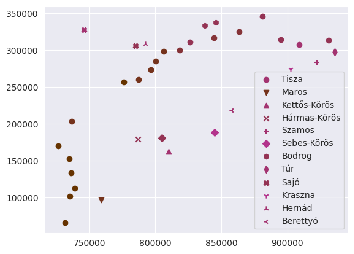
\includegraphics[width=7.4370818575364cm,height=5.62314705496524cm]{protocol-5.pdf}}
  \caption{Graph: x-axis: $i$, y-axis: $c_i$ for a Station, $p_{\tmop{val}}
  (t_X) \ll 10^{- 3}$, 2004-2006}
\end{figure}

\

If we now visualize $t_X$ for every station on a map, we can see if the
results appear to make sense. Stations further upstream take longer to
influence the water levels in Szeged.

\begin{figure}[h]
  \raisebox{0.0\height}{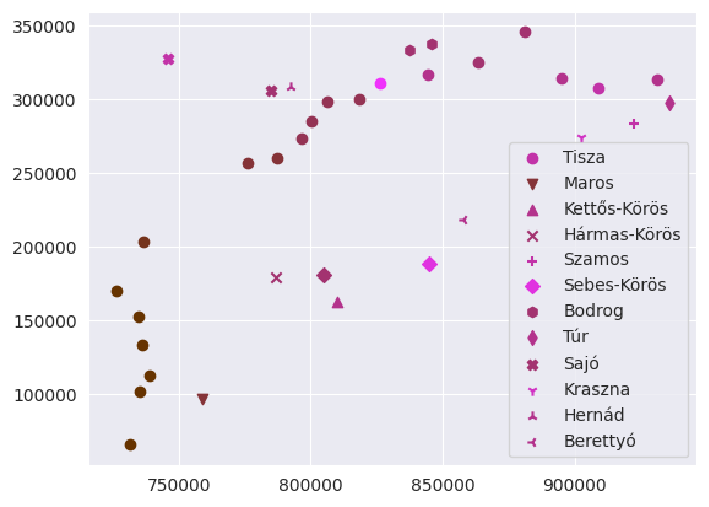
\includegraphics[width=11.899334251607cm,height=8.51915256460711cm]{protocol-6.pdf}}
  \caption{Stations colorized by $t_X$}
\end{figure}

Note: The light dot along the Tisza is right at one of the dams.

\subsubsection{Other correlation measures}

In the procedure described above we initially used the regular Pearson
correlation. We then repeated the procedure with Spearman and Distance
correlation. We got similar results:

\tmfloat{h}{small}{figure}{\raisebox{0.0\height}{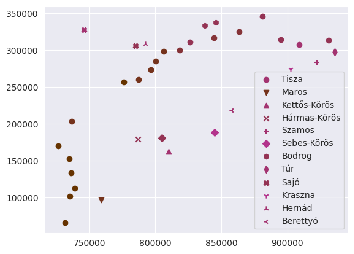
\includegraphics[width=5.94965892693165cm,height=4.25955988455988cm]{protocol-7.pdf}}}{Map,
Spearman
Correlation}\tmfloat{h}{small}{figure}{\raisebox{0.0\height}{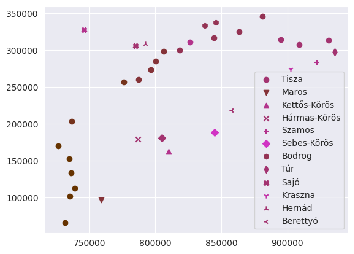
\includegraphics[width=5.94965892693165cm,height=4.25955988455988cm]{protocol-8.pdf}}}{Map,
Distance Correlation}

\subsubsection{Correlation $\neq$ Causality}

In general, correlation does not imply causality. However, since we are
looking at a river we know there exists at least some level of causality since
water flows downstream. The results we measured via correlation, also support
this direction of informational flow. We even found, that stations downstream
of Szeged show negative delay, further supporting the validity of the test
performed above.

\subsubsection{Conclusion}

With each correlation measure we got similar results. Except for less than a
handful of stations, their maximally correlated delay was 7 days or less. So
dropping stations, with the suggested argument of them being too far away, did
not work.

\subsection{Choosing Models}

We mainly considered 3 different models.
\begin{enumerateroman}
  \item The {\tmstrong{LSTM}} (= Long-Short Term Memory) takes the water level
  data of a single day, as well as its memory, as an input and outputs its new
  memory for the next day. This is run recursively multiple times. On the last
  day the network makes a prediction for the next seven days.
  
  \item One could use a {\tmstrong{CNN}} (= Convolutional Neural Network)
  which convolutes over the time dimension of the input. This way the CNN
  might be able to ``see'' flood waves coming. Whereas the LSTM has to
  mentally keep track of them.
  
  \item Seven {\tmstrong{fully dense NNs}} that each take only a single
  measurement per station as an input and each provide a prediction for a
  single day in the forecast.
\end{enumerateroman}

\subsection{Implementation}

All the models were implemented in a PyTorch environment. In the process of
making the prediction, using a neural network, a critical step is the data
modification and split. In the case of all the models, fifteen days of data
from the past was used to predict the following seven days. So the data should
be fed to the networks as an input of a $15 \times K$-sized matrix (where $K$
is the number of stations used) and the ground truth data of the following
predicted days are a seven-number long vector representing the water levels in
Szeged.

In the topic of neural networks, one genuinely significant aspect of learning,
is the manipulation of the data. We already applied the steps described in
chapters \ref{clean} to \ref{imputation}. Furthermore the data should be
standardized, having only a smaller region of input and output data. In the
most cases, the standardization means using zero means and unit standard
deviation by subtracting the mean of the training data from all data and
dividing by the standard deviation of the training data. Which needs to be
done for each station separately. It is highly important to use only the
training set for determining the mean and standard deviation values, in other
cases some validation information can be added to the network, which can cause
look-ahead bias.

After the data preprocessing is done, the models can be built.

\subsubsection{LSTM}

The LSTM model consists of an LSTM layer, followed by a linear layer at the
end. The hyperparameters of the model are ten hidden sizes for the five LSTM
layers. The linear one is used only for subtracting the result from these
layers, using ten input and seven output neurons.

\subsubsection{CNN}

The first CNN approach uses only an arbitrary order of stations and an
one-dimensional convolution along the dataset, so the convolution kernel is
only shifted along the time dimension and uses the data from all chosen
stations, added as different channels to the model. There are five-, nine- and
three-sized kernels being used respectively, by the seven hidden channels,
each separated by a ReLU activation function.

In the case of this model, the network has to understand the spatial
information inside the data, because all the stations, in an arbitrary order,
get passed to the network, so there is no information added to the network in
connection with how fast the water level difference is propagated to Szeged.
So, the CNN should use the spatial information as well. To do that, the new
dataset is arranged using the causality information in a way, that on the left
Szeged and stations with maximal zero-day difference is indicated and going
towards the right side of the table, more days take the water affecting Szeged
station. This is fed to the network in a form, that in the first convolution
layer only the closest stations are added to the network as channels,
{\tmstrong{after day the stations being one day far away Szeged,}} followed by
two day one{\ldots} using seven blocks at the end. The last block contains not
only the stations which are eight days away, but all the remaining ones as
well. This way the network gets new information at every step whilst
processing the old information as well. In the end, the above-described CNN is
ended to process all the information.

\subsubsection{Dense NN}

A dense neural network was also built using one-day data from all the
stations. The used day was determined by the spatial information, so always
the most significant day was added to the network. In order to keep the task
simple, for a fully dense linear network, only one-day prediction was used,
and seven different networks were built to predict all seven days. This
network is not further mentioned because the results were much worse than the
baseline model.

\subsubsection{Custom loss functions}

Another highly significant part of building a neural network is deciding what
kind of loss function is used. We tried several kinds of functions. At first,
the widely used L2 loss function, which is the mean square error between the
ground truth and the prediction. The test showed that using this many stations
will give inaccurate results for the first few days but relatively good ones
for the end. To make the network focus better the following days ahead, the
first idea was to use a weighted mean square error, having linear or squared
weights, by dividing the difference by the number of days being ahead of the
current one or by the square of them.

The network should perform well, not only in everyday cases but also when
floods occur. This can be done by giving a bigger punishment to the network
for not being precise when the water level is higher. The custom loss
functions are the following:
\begin{itemizedot}
  \item ReLU function giving a smaller weight in the case of the difference is
  under a specific water level and after that a linearly increasing weight.
  
  \item ReLU function with the same property described above but using not a
  linear but a squared increase.
  
  \item Using a sigmoid-like function, built from two different parabolas.
  
  \item Staircase function, giving increasing weight as the water level grows.
  
  \item Two squared ReLU functions, one for the positive and one for the
  negative x-axis. This is the variant we use when talking about a custom loss
  function in the following chapters.
\end{itemizedot}
{\noindent}\begin{tabularx}{1.0\textwidth}{cc}
  \tmfloat{h}{small}{figure}{\raisebox{0.0\height}{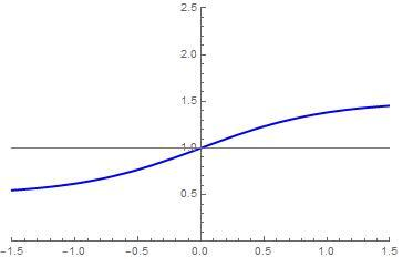
\includegraphics[width=6.69337859110586cm,height=4.35068214613669cm]{protocol-9.pdf}}}{custom
  loss, ReLU} &
  \tmfloat{h}{small}{figure}{\raisebox{0.0\height}{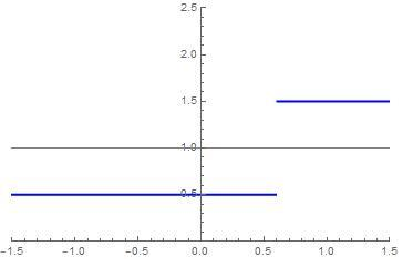
\includegraphics[width=6.69337859110586cm,height=4.35068214613669cm]{protocol-10.pdf}}}{custom
  loss, squared ReLU}\\
  \tmfloat{h}{small}{figure}{\raisebox{0.0\height}{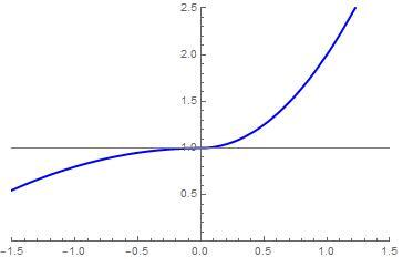
\includegraphics[width=6.69337859110586cm,height=4.35068214613669cm]{protocol-11.pdf}}}{custom
  loss, sigmoid} &
  \tmfloat{h}{small}{figure}{\raisebox{0.0\height}{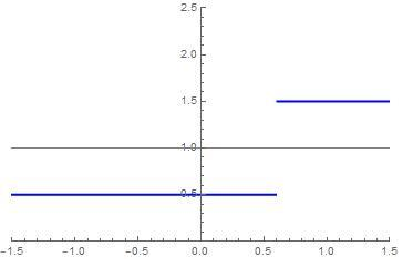
\includegraphics[width=6.69337859110586cm,height=4.35068214613669cm]{protocol-12.pdf}}}{custom
  loss, staircase}\\
  \tmfloat{h}{small}{figure}{\raisebox{0.0\height}{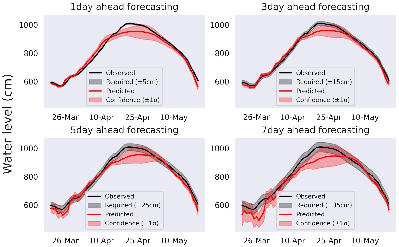
\includegraphics[width=6.69337859110586cm,height=4.35068214613669cm]{protocol-13.pdf}}}{custom
  loss, double squared ReLU} & \ 
\end{tabularx}

\subsubsection{Learning rate}

To have the best results from the networks possible, a learning rate
scheduler, which reduces the learning rate in the case of reaching a plateau,
was added to the network. We used Adam optimizers and early stopping with ten
epochs of patience. All the models were trained in five hundred epochs (but
they stopped before then, because of the early stopping feature). The used
batch size was eight.

\

\subsection{Verification of Results}

We utilized four distinct metrics for the verification of our models. The code
employed for this purpose is largely adapted from the existing verification
code provided by our instructor. The validation dataset, spanning from 2005 to
2020, was employed for this analysis.

The metrics encompassed the Mean Absolute Error (MAE), offering insights into
error magnitudes, and the Root Mean Square Error (RMSE), which emphasizes
outliers more than MAE. Additionally, we computed $R^2$ values and employed
Willmott's Index (WI). For the MAE and RMSE values near 0 indicate a better
fit. For the $R^2$ and the WI values close to 1 are preferable.

Our analysis extended to evaluating deviations from the required confidence
interval of $5 \text{cm}$ over a 5-day period for each model. The results were
visualized through scatterplots and tables. Moreover, we examined how the
models performed during flood conditions, specifically focusing on the 2006
and 2013 floods. This involved generating line plots that compared model
predictions against observed values for the given time period. As a further
comparison we also checked a timespan with medium to low water leves, during
June and July of 2007.

\section{Discussion}

The above-described models were compared to each other and two other models,
baseline and the best performing LSTM model from the given
paper{\cite{WaterLevel2023}}. The results were compared with the same metrics
described in the paper. Using MAE, RMSE, R2 and WI metrics, the same result
can be seen. For the first-day prediction, our models underperform the
baseline model. However, our LSTM and simple CNN give a better result after
the fourth day of prediction. An interesting behavior can be seen in the case
of the spatial CNN because it gave worse results than the baseline model in
the case of the first and last two days. But having an overall view is not
enough in our case. A good model can predict well not only on average but in
the case of a flood as well.

\

\begin{figure}[h]
  \raisebox{0.0\height}{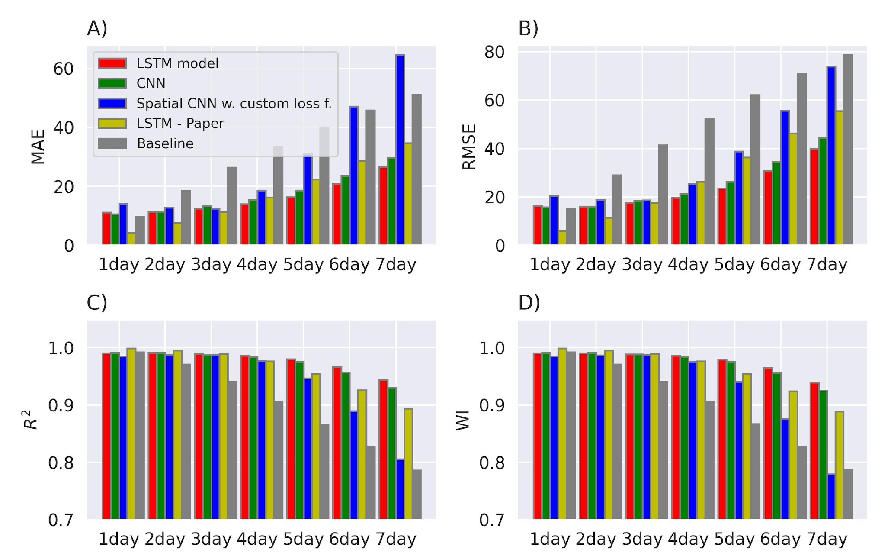
\includegraphics[width=14.8741637150728cm,height=9.38961038961039cm]{protocol-14.pdf}}
  \caption{Results, different metrics}
\end{figure}

\

Using the flood from the validation data we can see that the LSTM network
cannot reach the top of the water level in a case of prediction in the first
three days, but it barely reaches the given required interval using one sigma
confidence interval for the fifth and seventh day. Though, on average the LSTM
network outperformed the simple CNN one, it managed to reach the given
required region in the case of a flood. Using spatial information, the same
well-performing result can be seen with a smaller confidence interval. The CNN
interval shrank the deviation of the data.

{\noindent}\begin{tabularx}{1.0\textwidth}{@{}X@{}@{}X@{}}
  \tmfloat{h}{small}{figure}{\raisebox{0.0\height}{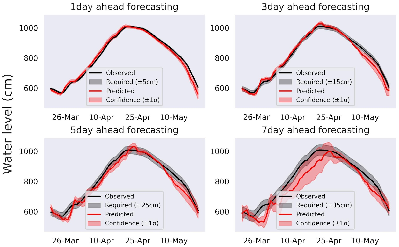
\includegraphics[width=6.69337859110586cm,height=4.14413616686344cm]{protocol-15.pdf}}}{2006
  flood prediction, LSTM} &
  \tmfloat{h}{small}{figure}{\raisebox{0.0\height}{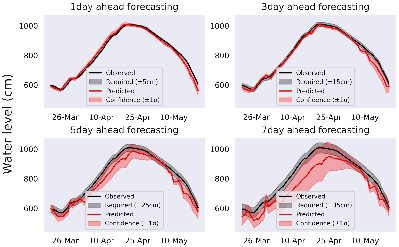
\includegraphics[width=6.69337859110586cm,height=4.14413616686344cm]{protocol-16.pdf}}}{2006
  flood prediction, CNN}\\
  \tmfloat{h}{small}{figure}{\raisebox{0.0\height}{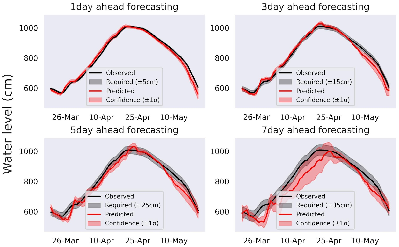
\includegraphics[width=6.69337859110586cm,height=4.14413616686344cm]{protocol-17.pdf}}}{2006
  flood prediction, custom loss CNN} &
  \tmfloat{h}{small}{figure}{\raisebox{0.0\height}{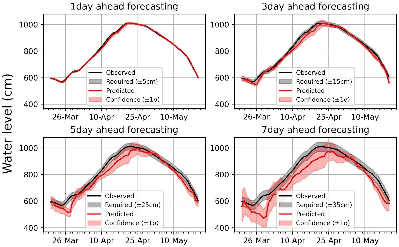
\includegraphics[width=6.69337859110586cm,height=4.14571035025581cm]{protocol-18.pdf}}}{2006
  flood prediction, paper{\cite{WaterLevel2023}}}
\end{tabularx}

\section{Conclusion}

The main difference between our method and the one described in the
paper{\cite{WaterLevel2023}}, is, that we used information, collected by many
more stations, for predicting the model but smaller and simpler models as
well. As we can see in the results, using more stations helps in the
prediction for the future. We managed to outperform the paper's network after
day four, but the prediction was poor, for the first day, even worse than a
baseline model.

\section{Group work dynamics}

During the modelling week, our group participated in meaningful and productive
communication. Due to the evolving nature of the project, it was not possible
to plan far ahead, and the work was distributed afresh every day. First thing
in the morning, we started with brainstorming new ideas and distributing the
work. It quickly crystallized itself which tasks suited everyone best. While
Bal{\'a}zs Endr{\'e}sz and Lorenz Auer mostly worked on the machine learning
models, Aleksis Tammi and Endre Mitlas{\'o}czki worked on both data
visualization and the models. Franz Scharnreitner was working on data analysis
and imputation. Thus, the work was evenly split, and the group was able to
work without much downtime.

During brainstorming, the group had a multitude of ideas, and it was a
challenge to filter out the ones that were worth pursuing and manageable
within the timeframe of a week. The group handled this challenge very well,
although there were still many ideas left behind, that could have been
implemented if there was more time to work together.

Sharing code was achieved both through GitHub and Google Colab. Both tools
worked well, and we did not have any problems with files not being shared or
version conflicts.

\section{Instructor's assessment}

The work with the team was arranged as an R$\&$D project is structured in the
industry. In the morning of the first day, we had a detailed discussion about
the topic of the problem: scientific background, data collection methods,
structure of the data, previous results and goals for the week. They showed
great attention and raised good questions already in the very first
discussion, which gave me a good impression about the participants. We planned
with three further catch-up sessions during the week (Monday, Wednesday and
Friday afternoons), but we had short discussions every day, since they had
several, equally promising and creative ideas about data processing and model
building, thus I was eager to have more sessions with them.

None of them were an expert in machine learning algorithms applied for time
series (which is a complex topic), but they were able to ramp up the required
knowledge in a short period of time: this skill will be very valuable at their
work in the industry. I was also satisfied with their ability for system
understanding, which led to have good and creative improvement ideas at
different steps of the machine learning pipeline (data imputation, ML model
architecture, loss functions) even in the early stage of the work. Despite
there were some flawed or not well thought ideas during the week, we could
discuss the problematic points all the time and they were improved them until
the next meeting.

Since this project was really implementation-heavy, fortunately everybody was
familiar with programming in the necessary level and there were leaders in the
coding of the larger blocks of the code. They got used to programming in a
collaborative manner in short time, which spared a lot of time for them and
this enabled them to try a lot of ideas and execute several model trainings. I
was satisfied to see that they can use and build into their code the
previously developed research code without bigger issues.

It was clear from the second day, that they were able to discuss the strengths
of the individual members of the group and they could distribute very quickly
the work of the complex task, which indicated their capability for teamwork.
As I have seen there was no real conflict in the team: if someone was
responsible for a concept or code, he explained the details, but it was clear
that everybody played a part in that specific part. They could also prove
their excellent teamwork at the presentation of the Modelling Week, where
everybody contributed to the talk.

In summary, I was very satisfied with their work they did during the intensive
5 days of the ECMI Modelling Week. They implemented good improvement ideas for
water level prediction and they were able to outreach the previous performance
results for later days of the prediction. In my opinion, they got a complete
picture about data-driven algorithm development in a team, which is a fruitful
experience for their later career in this field.

\section{Links}

Google Colab:
\href{https://colab.research.google.com/drive/1ZobMWBW76xJHmeTsbXmjmgCzcv5sGrSV?usp=sharing}{work
notebook and LSTM}

Google Colab:
\href{https://colab.research.google.com/drive/1TM0TM2p8cphnl7WuYu9bTIFMF2lW8gyv?usp=sharing}{CNN}

\begin{thebibliography}{1}
  \bibitem[1]{WaterLevel2023}\label{docs-internal-guid-0a5e5cca-7fff-6f48-cf8a-a203f7614dd1}Zsolt
  Vizi, B{\'a}lint Batki, Luca R{\'a}tki, Szabolcs Szal{\'a}nczi, Istv{\'a}n
  Feh{\'e}rv{\'a}ry, P{\'e}ter Koz{\'a}k, T{\'i}mea Kiss. {\newblock}Water
  level prediction with various machine learning algorithms for a lowland
  river. {\newblock}2023.{\newblock}
\end{thebibliography}

\end{document}
